\section{MOTION PLANNING}
\label{sec:motion-planning}

To design a motion planning method that minimizes psychological discomfort when a flapping drone approaches a human, we must consider the several factors:

\subsection{Distance}
\label{sec:distance}
Given the expected size and shape of a flapping drone, we estimate that the minimum acceptable distance falls within a specific range. By maintaining this distance while gradually invading the landing zone, the psychological burden can be minimized.
Several studies have investigated the psychological burden imposed by drones depending on their distance from humans useing different drone sizes\cite{Yeh2017Proxemics, lieser2021evaluating-distances,Duncan2013comfortable-approach, Acharya2017robot-vs-drone-comfort}.
\cite{lieser2021evaluating-distances} is a paper focusing on tactile drone interaction using a drone with a wheelbase of 0.92m, which is suitable for palm landing.
This paper conducted an experiment in which participants were asked to stop the drone when they felt uncomfortable by using foot (non-contact) and hand (contact) methods.
The results show that the overall stop distance was $\bar{x}$ = 0.63m ($\sigma$ = 0.33m),
which means that, if the drone needs to approach closer than this distance, it should be done in psychologically safe manners such as gradually decreasing the speed or using a trajectory that does not directly approach the user so that the user does not feel threatened.

Moreover, the study \cite{lieser2021evaluating-distances} also shows that the average distance at which participants stopped the drone using their hands was $\bar{x}$ = 0.47m ($\sigma$ = 0.09m).
This indicates that physical contact should occur outside this range to guarantee physical and psychological safety.

\subsection{Altitude}

In the study \cite{lieser2021evaluating-distances}, the height was set to enable a convenient way of tactile interaction 
by allowing the participants to slightly look down to the quadrotor.
We follow this setting because then users do not need to move their head to look up to the drone and are able to simultaneously observe both the drone and their own hand, 
which leads to easier adjustmunts of the hand position while the drone is approaching.
Assuming that users lift their hand to the height of their elbow for palm landing, the drone should be positioned at the height of between the elbow and the eye level.

\subsection{Approach Direction}

As noted in \cite{lieser2021evaluating-distances}, the approach direction of the drone affects the psychological burden.
The study shows that the participants felt most uncomfortable when the drone approached them from the back because they could not see the drone.
Therefore, the drone should approach the user from the front or side to minimize the psychological burden.


\subsection{Velocity}

To assess the appropriate velocity of the drone, we need to consider the human perception of speed of an approaching object.
The study \cite{Kolling2012weber-fechner-law} shows that the drivers' perception of the speed of an foregoing vehicle follows Weber's Law:

\begin{equation}
    k{\Delta {\rm W}\over W}=\Delta s
\end{equation}

where $W$ is the measurable stimuli, $s$ the intensity of sensation, $\Delta$ the increment of physical quantity ($W$) and sensation intensity ($s$), and $k$ the coefficient. 
In the study \cite{Kolling2012weber-fechner-law}, $W$ corresponds to the the distance between the cars and $s$ to the speed of the driver's car.
We assume that the same law can be applied to the perception of the speed of an approaching drone by regarding the distance between the drone and the user as $W$ and the perceptive speed of the drone as $s$.
This assumption explanes the result of the previous study on perceived safety of drones \cite{van2023perceived-safety}, 
which shows the trend that larger distances are perceived as overly safe while a fast-moving drone close to participants is perceived as less safe than needed,
because we can consider from the law that the participants perceive the speed of the drone as too slow due to the large distance between the drone and the participants and as too fast due to the short distance between the drone and the participants.
Denoting the speed of the drone as $v$, the distance between the drone and the user as $d$, and time as $t$, we can derive the following equation:

\begin{equation}
    k{v\Delta t\over d}=\Delta s
\end{equation}

To secure the psychological safety, the drone should approach the user keeping $\Delta s$ constant.
Thus, the speed can be caliculated as follows:

\begin{equation}
    v = {k^\prime d\over \Delta t}
    \label{eq:speed}
\end{equation}

where $k^\prime$ is a constant.

\subsection{Trajectory Design}
\label{sec:trajectory}

\begin{figure}[t]
    \centering
    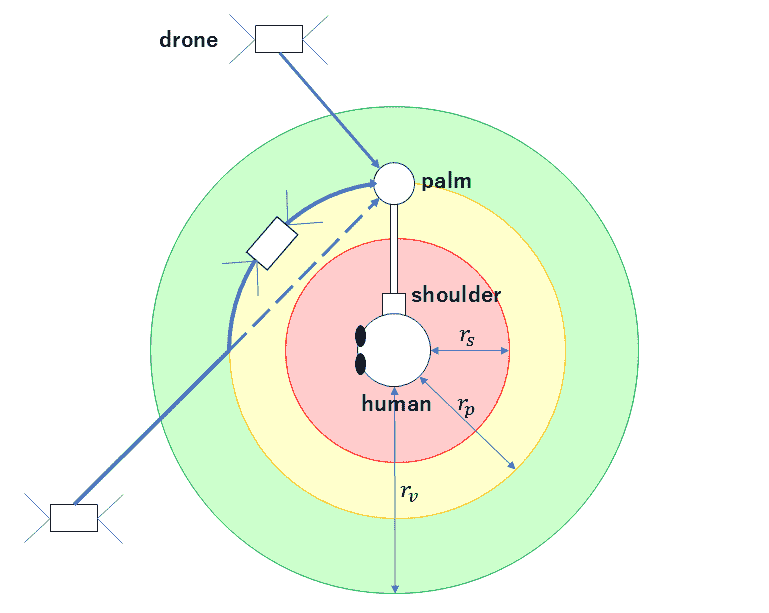
\includegraphics[width=\columnwidth]{motion-planning.png}
    \caption{Proposed motion planning for flapping drone approach. It has 4 domains which are separated by the distance from the user. Different strategies are applied to drone motion in different domains.
    }
    \label{fig:trajectory}
\end{figure}

Based on the above findings, we propose the following motion planning method, as illustrated in Figure \ref{fig:trajectory}.
We divide the approach trajectory into four domains based on the distance between the drone and the user $r$.

\begin{enumerate}
    \item $r > r_v$
    
    The drone is far from the user and approaches the palm straight at a constant speed.
    We let $r_v$ = 0.63m based on \ref{sec:distance}.

    \item $r_v \geq r > r_p$
    
    The drone is close enough to the user to be possibly perceived as unsafe, so it gradually decreases its speed by following (\ref{eq:speed}).

    \item $r_p \geq r > r_s$
    
    The drone is inside the circle with the radius of user's arm length $r_p$ centered at the user's chest.
    To maintain a certain distance from the user, the drone moves along the circle toward the user's palm while decelearting.
    On this path, the velocity of the drone towards the user's chest is always zero,
    which means $\Delta s$ = 0 in (\ref{eq:speed}) and minimizes the threat to the perceived safety.

    \item $r \leq r_s$
    \label{sec:innermost}
    
    If the drone is within this range, it is too close to the user and has a high risk of collision.
    Thus, the drone avoids the user by moving away from the user's body.
    Moreover, if the palm is within this range, the drone stays still and waits for the user to move their palm to the landing position outside the range so that the drone will not intrude the domain.
    We let $r_s$ = 0.47m based on \ref{sec:distance}.

\end{enumerate}